\documentclass{standalone}
\usepackage{tikz}
% remover comentários -> apagar o '%'
% ATIVIDADE 1
%\usetikzlibrary{calc}


\begin{document}
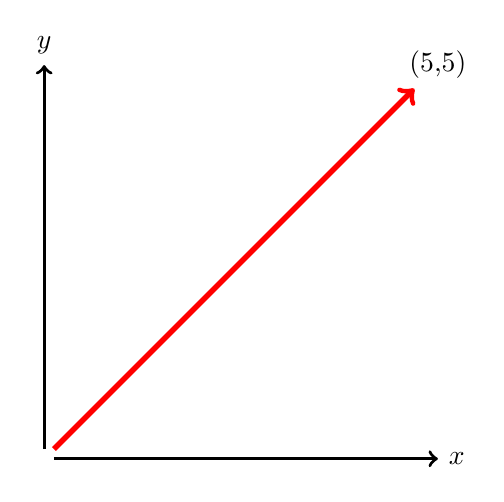
\begin{tikzpicture}

	\def \xmax{5};
	\def \ymax{5};

	\node[anchor=center, fill=none] (origemXY) at (0,0) {};
	\node[anchor=center] (fimXY) at (\xmax, \ymax) {(\xmax,\ymax)};
	
	\draw[very thick, ->, anchor=southh west] (origemXY) -- (0,\ymax) node(yaxis)[above] {$y$};
	\draw[very thick, ->, anchor=north west] (origemXY) -- (\xmax, 0) node(xaxis)[right] {$x$};
	
	\draw[->, color=red, line width=2pt] (origemXY)--(fimXY) {} ;
	
	
	\def \myXYOx{1};
	\def \myXYOy{2};

	\def \myXYFx{3};
	\def \myXYFy{4};
	
	% ATIVIDADE 1
	%\draw[->, color=blue, dashed, line width=1pt] ($(origemXY)+(\myXYOx,\myXYOy)$)--($(origemXY)+(\myXYFx,\myXYFy)$) node(myvec)[right] {(\myXYFx,\myXYFy)} ;

	% ATIVIDADE 2
	%\draw[<->, color=orange, line width=5pt] ($(origemXY)+(3,0.5)$)--($(origemXY)+(4,7*0.22)$) node(myvec2)[below, text width=2cm, yshift=-0.10cm, xshift=0.15cm, text centered, rotate=45] {qualquer \\ coisa} ;
	
	% ATIVIDADE 3
	%\coordinate (mypoint) at (1,4);
	%\coordinate (mypointR) at ($(mypoint)+(1,0)$);
	%\node[minimum width=1mm, minimum height=1mm, fill=blue] (mydot) at (mypoint) [] {};
	%\node[minimum width=1mm, minimum height=1mm, fill=green, rotate=45] (mydotrotated) at (mypointR) [] {};
	%\node[] (mydottext) at (mypoint) [below] {dot};
	
\end{tikzpicture}

\end{document}
